%%%%%%%%%%%%%%%%%%%%%%%%%%%%%%%%%%%%%%%%%
% Beamer Presentation
% LaTeX Template
% Version 1.0 (10/11/12)
%
% This template has been downloaded from:
% http://www.LaTeXTemplates.com
%
% License:
% CC BY-NC-SA 3.0 (http://creativecommons.org/licenses/by-nc-sa/3.0/)
%
%%%%%%%%%%%%%%%%%%%%%%%%%%%%%%%%%%%%%%%%%

%----------------------------------------------------------------------------------------
%	PACKAGES AND THEMES
%----------------------------------------------------------------------------------------

\documentclass[tikz,table,border=2mm]{beamer}
\usepackage{hyperref}
\usepackage{listings}
\usepackage{tikz}
\usepackage{PTSansNarrow}
\usepackage[T1]{fontenc}
\usepackage{array,tabularx}
\usepackage[most]{tcolorbox}
\usepackage{url}
\usepackage{animate}

\setbeamertemplate{itemize/enumerate subbody begin}{\tiny}

\mode<presentation> {

% The Beamer class comes with a number of default slide themes
% which change the colors and layouts of slides. Below this is a list
% of all the themes, uncomment each in turn to see what they look like.

%\usetheme{default}
%\usetheme{AnnArbor}
%\usetheme{Antibes}
%\usetheme{Bergen}
%\usetheme{Berkeley}
%\usetheme{Berlin}
\usetheme{Boadilla}
%\usetheme{CambridgeUS}
%\usetheme{Copenhagen}
%\usetheme{Darmstadt}
%\usetheme{Dresden}
%\usetheme{Frankfurt}
%\usetheme{Goettingen}
%\usetheme{Hannover}
%\usetheme{Ilmenau}
%\usetheme{JuanLesPins}
%\usetheme{Luebeck}
%\usetheme{Malmoe}
%\usetheme{Marburg}
%\usetheme{Montpellier}
%\usetheme{PaloAlto}
%\usetheme{Pittsburgh}
%\usetheme{Rochester}
%\usetheme{Singapore}
%\usetheme{Szeged}
%\usetheme{Warsaw}

% As well as themes, the Beamer class has a number of color themes
% for any slide theme. Uncomment each of these in turn to see how it
% changes the colors of your current slide theme.

%\usecolortheme{albatross}
%\usecolortheme{beaver}
%\usecolortheme{beetle}
%\usecolortheme{crane}
%\usecolortheme{dolphin}
%\usecolortheme{dove}
%\usecolortheme{fly}
%\usecolortheme{lily}
%\usecolortheme{orchid}
%\usecolortheme{rose}
%\usecolortheme{seagull}
%\usecolortheme{seahorse}
%\usecolortheme{whale}
%\usecolortheme{wolverine}

%\setbeamertemplate{footline} % To remove the footer line in all slides uncomment this line
%\setbeamertemplate{footline}[page number] % To replace the footer line in all slides with a simple slide count uncomment this line

%\setbeamertemplate{navigation symbols}{} % To remove the navigation symbols from the bottom of all slides uncomment this line
}

\usepackage{graphicx} % Allows including images
\usepackage{booktabs} % Allows the use of \toprule, \midrule and \bottomrule in tables

%----------------------------------------------------------------------------------------
%	TITLE PAGE
%----------------------------------------------------------------------------------------

\title[Computer vision crash course]{Introduction to computer vision : from OpenCV to YOLO} % The short title appears at the bottom of every slide, the full title is only on the title page

\author{Damien Meur} % Your name
\institute[PXC] % Your institution as it will appear on the bottom of every slide, may be shorthand to save space
{
Proxyclick \\ % Your institution for the title page
\medskip
\textit{dmeur@proxyclick.com} % Your email address
}
\date{\today} % Date, can be changed to a custom date

\begin{document}

\begin{frame}
\titlepage % Print the title page as the first slide
\end{frame}

\begin{frame}
\frametitle{Overview} % Table of contents slide, comment this block out to remove it
\tableofcontents % Throughout your presentation, if you choose to use \section{} and \subsection{} commands, these will automatically be printed on this slide as an overview of your presentation
\end{frame}

%----------------------------------------------------------------------------------------
%	PRESENTATION SLIDES
%----------------------------------------------------------------------------------------

%------------------------------------------------
\section{Setup}

\begin{frame}
\frametitle{Required tools}
\begin{itemize}
\item Python 3.6+
\item OpenCV 4.X+
\item TensorFlow 2.X
\item Jupyter 1.X+
\end{itemize}
\end{frame}

\begin{frame}
\frametitle{Links}
\begin{itemize}
\item Anaconda : \url{docs.anaconda.com/anaconda/install/}
\item GitHub repository : \url{github.com/damioune123/computer_vision_crash_course}
\end{itemize}
\end{frame}

\begin{frame}
\frametitle{Installation with anaconda}
\lstinputlisting[language=Bash]{code/anaconda_install.sh}
\end{frame}

\section{What is computer vision ?}
\begin{frame}
\frametitle{What is computer vision ?}
\begin{itemize}
	\item The human brain is amazingly good at \textbf{detecting and classifying objects}, a large part of our brain is dedicated to vision (occipital lobe).
	\item \textbf{CV} is a collection of machine learning techniques that makes computer mimic these two specific tasks.
	\item How a computer would do this task that is so easy to us though ? First let's dig into how a computer "sees".
\end{itemize}
    \begin{figure}
    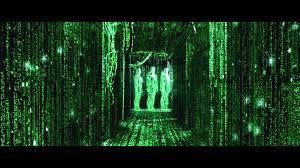
\includegraphics[width=0.6\linewidth]{images/matrix.jpeg}
    \end{figure}
\end{frame}


\subsection{Numeric image representation}


\begin{frame}{Numeric image representation}
    \begin{figure}
    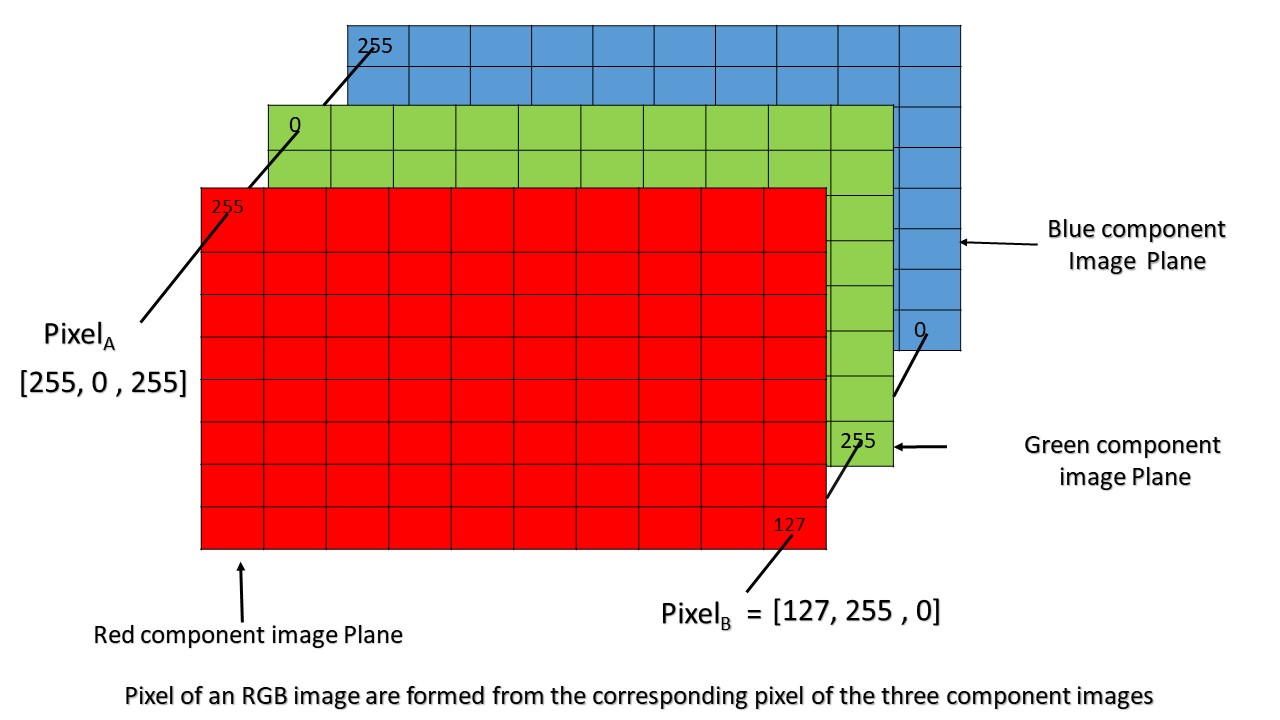
\includegraphics[width=0.8\linewidth]{images/pixel.jpg}
    \end{figure}
    
    \begin{block}{What are images ?}
        Basically a matrix of pixels, each pixel is represented by 3 color (RGB) values (0-255)
    \end{block}


\end{frame}

\begin{frame}{Numeric image representation}
Is it possible to use these raw values directly to detect or classify objects ?
\begin{alertblock}{No}
    Let's take an average image  (3.1 Megapixels resolution) :
    \begin{itemize}
	\item  2048 X 1536 pixels => 3,145,728 pixels.
	\item X 3 color channels => 9,437,184 parameters !
	\end{itemize}
\end{alertblock}
Could we simplify the problem ?
\begin{block}{Yes}
By keeping only the relevant information (\textbf{feature extraction}). Bearing in mind there is a trade-off acccuracy vs performance.
\end{block}

\end{frame}
\subsection{Different technical approaches : old machine learning vs new deep learning techniques}
\begin{frame}{Different technical approaches : old machine learning vs new deep learning techniques}
    \begin{figure}
    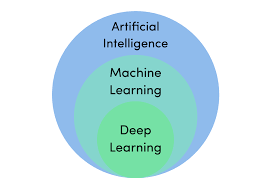
\includegraphics[width=0.6\linewidth]{images/ml_vs-dl_2.png}
    \end{figure}
\end{frame}
\begin{frame}{Different technical approaches : old machine learning vs new deep learning techniques}
    \begin{figure}
    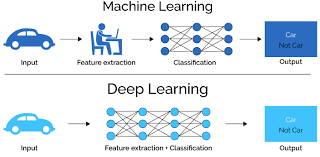
\includegraphics[width=0.5\linewidth]{images/ml_vs-dl_1.png}
    \end{figure}
    \begin{figure}
    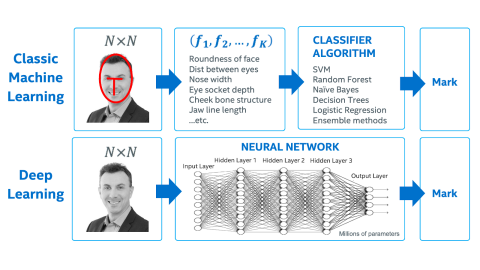
\includegraphics[width=0.5\linewidth]{images/ml_vs_dl_1.png}
    \end{figure}
\end{frame}

\begin{frame}{Different technical approaches : old machine learning vs new deep learning techniques}
\rowcolors{1}{black!25}{white}
\begin{tcolorbox}[enhanced, notitle, clip upper, fontupper=\sffamily,%
    tabularx={>{\cellcolor[gray]{.5}\color{white}}r%
              >{\centering\arraybackslash}X%
              >{\centering\arraybackslash}X}]
  &\cellcolor{black!80}\color{white}HAAR-like features cascade classifiers &\cellcolor{black!80}\color{white}YOLO deep network \\
Single-class object detection accuracy & Good & Very good \\
Single-class object detection performance & Excellent & Very good \\
Multi-class object detection accuracy & N/A & Very good \\
Multi-class object detection performance & N/A & Very good \\
Object classification accuracy     &  N/A & Very good  \\
Object classification performance     & N/A  & Very good \\

\end{tcolorbox}
\footnote{\href{https://www.baseapp.com/deepsight/opencv-vs-yolo-face-detector}{\nolinkurl{https://baseapp.com/opencv-vs-yolo-face-detector}}}
\footnote{\href{https://towardsdatascience.com/whats-the-difference-between-haar-feature-classifiers-and-convolutional-neural-networks-ce6828343aeb}{\nolinkurl{https://towardsdatascience.com/diff-between-yolo-and-haar}}}
\end{frame}

\begin{frame}{Different technical approaches : old machine learning vs new deep learning techniques}
\begin{block}{It seems HAAR cascade is obsolete...}
\url{https://www.youtube.com/watch?v=XkfSqOvJRIw}
\end{block}

\begin{block}{...But}
\begin{itemize}
	\item It's also easier to understand/implement
	\item Requires less resource (still widely used on embedded system such as cameras) \footnote{\url{https://www.youtube.com/watch?v=uEJ71VlUmMQ}}
\end{itemize}
\end{block}

I choose to present you 3 techniques in this order : 
\begin{itemize}
	\item HAAR cascade : face and eye detection program
	\item Custom convolutional network : Face mask detector
	\item YOLO : Use the pre-trained network to detect any common objects
\end{itemize}
\end{frame}


\section{Hands on OpenCV}
\begin{frame}{Hands on OpenCV}
    \begin{block}{OpenCV}
        \textit{Open Source Computer Vision Library} is a library of programming functions mainly aimed at real-time computer vision.
    \end{block}
\begin{itemize}
	\item Built with C++
	\item Python/Java/Octave/Matlab official interfaces
	\item Contains a lot of tools to do basic/advanced image processing
	\item Has built-in machine learning object detection algorithms such as HAAR cascade

\end{itemize}
\end{frame}

\subsection{Basic image manipulations}
\begin{frame}{Basic image manipulations}
Let's do some image manipulations on OpenCV to better understand this library 
\end{frame}

\subsection{Edge detection}
\begin{frame}{Edge detections}
\begin{block}{Edges}
	Edges are sudden discontinuities in an image. They hold a lot of information about what's in the image.
\end{block}
\begin{block}{Edge detection}
	Edge detection is a very important in computer vision : helps with finding contours. 
\end{block}
\begin{figure}
    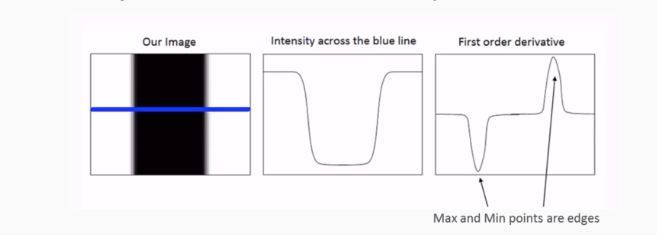
\includegraphics[width=1\linewidth]{images/edge_det_1.png}
\end{figure}
\end{frame}

\begin{frame}{Edge detection}
They are lots of different type of edge detection (all available in OpenCV)
\begin{itemize}
	\item Sobel : vertical or horizontal
	\item Laplacian : all orientations
	\item Canny (created by J.F Canny in 1986): optimal => low error rate, accurate (few noise detected as edge)
\end{itemize}
\end{frame}
\begin{frame}{Edge detection}
    \begin{figure}[ht]
        \begin{minipage}[b]{0.35\linewidth}
            \centering
            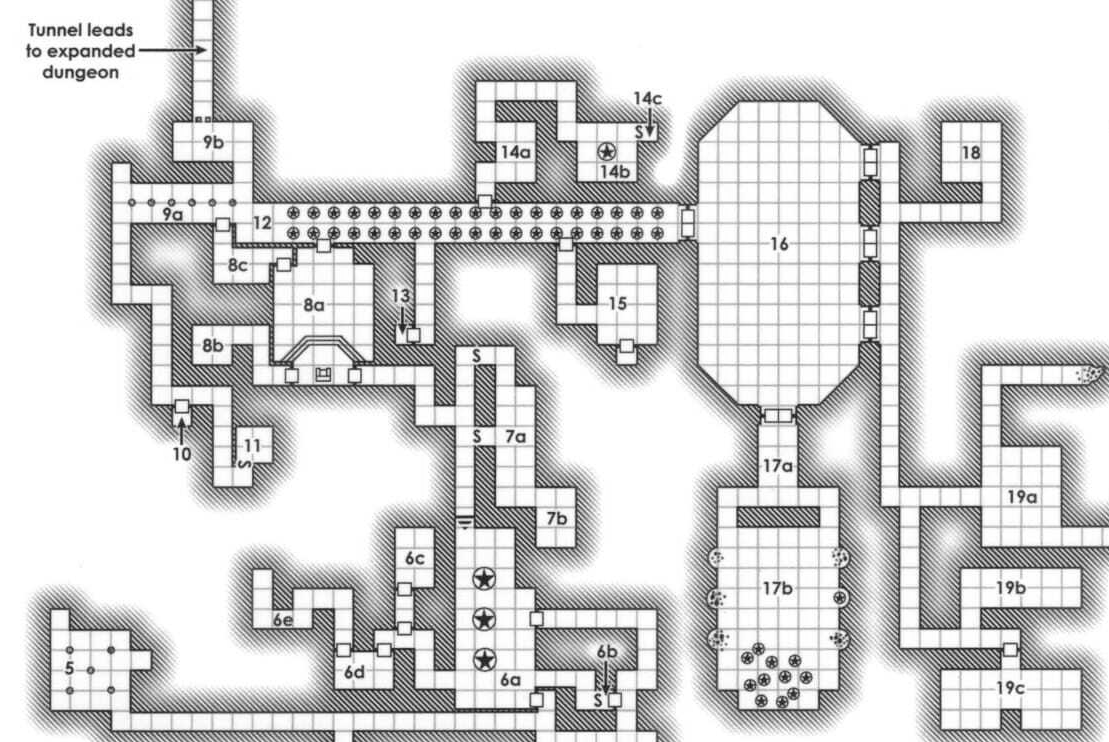
\includegraphics[width=\textwidth]{images/dungeon.png}
            \caption{Original}
            \label{fig:a}
        \end{minipage}
        \hspace{0.5cm}
        \begin{minipage}[b]{0.35\linewidth}
            \centering
            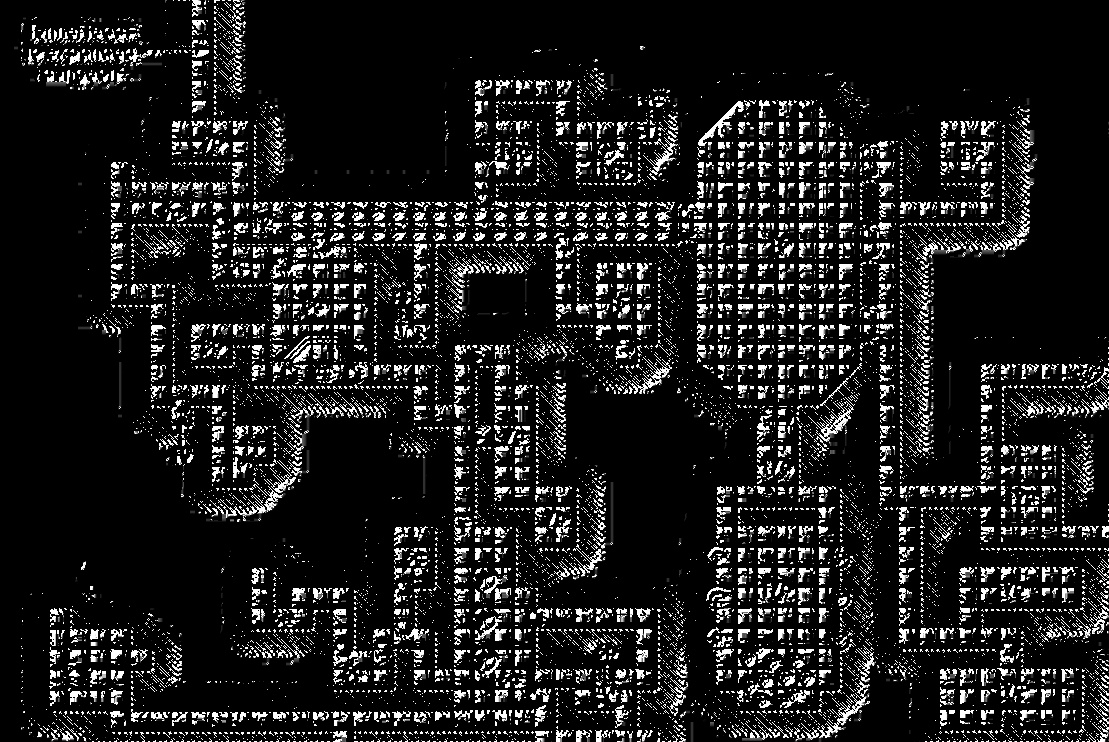
\includegraphics[width=\textwidth]{images/sobel_OR.jpg}
            \caption{Sobel (X + Y merged)}
            \label{fig:b}
        \end{minipage}
        \begin{minipage}[b]{0.35\linewidth}
            \centering
            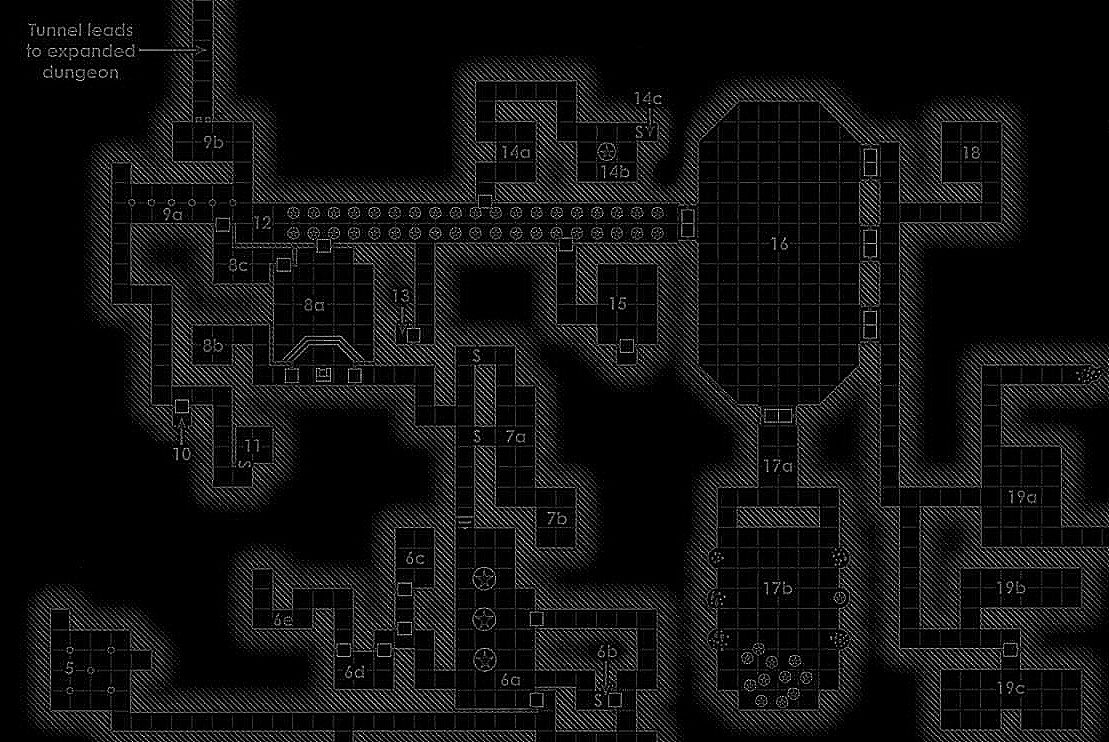
\includegraphics[width=\textwidth]{images/laplacian.jpg}
            \caption{Laplacian}
            \label{fig:a}
        \end{minipage}
        \hspace{0.5cm}
        \begin{minipage}[b]{0.35\linewidth}
            \centering
            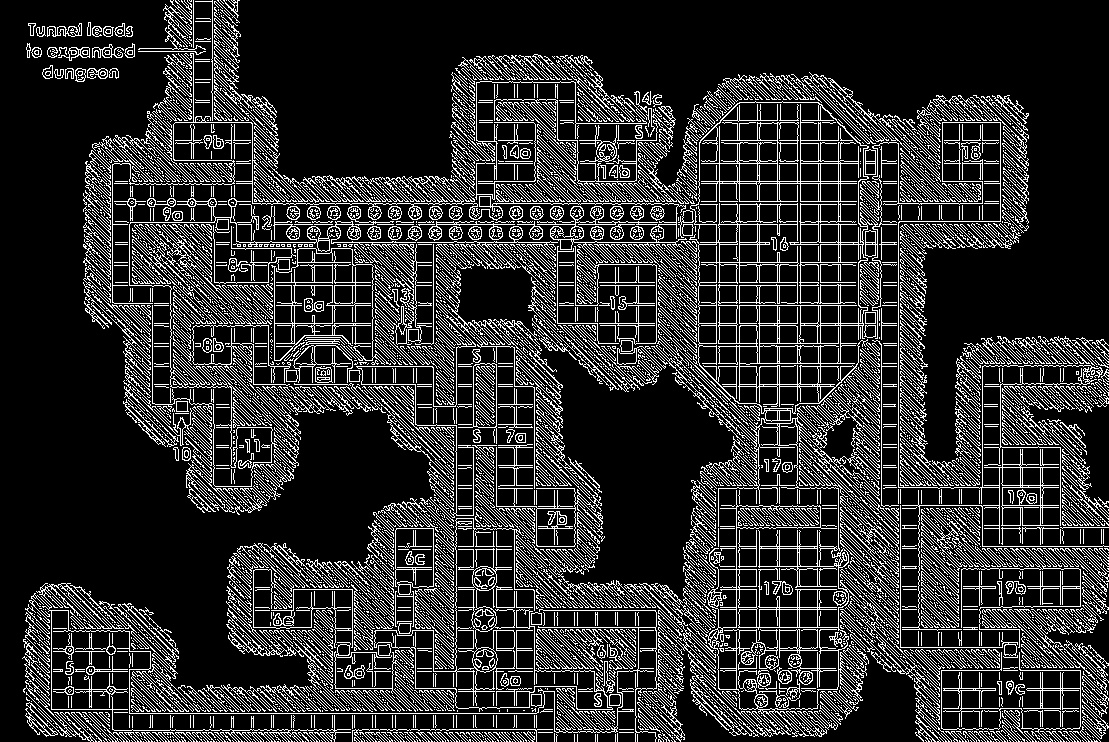
\includegraphics[width=\textwidth]{images/canny.jpg}
            \caption{Canny}
            \label{fig:b}
        \end{minipage}
    \end{figure}
\end{frame}
\begin{frame}
\frametitle{Edge detection}
\lstinputlisting[language=Python]{code/edge_detection.py}
\end{frame}

\begin{frame}{Edge detection}
Combine edge detection with a few OpenCV operations like bitwise operator, intensity threshold, opening (not detailed in this presentation) and you get ...\footnote{Code available in the jupyter notebook though}
\begin{figure}
    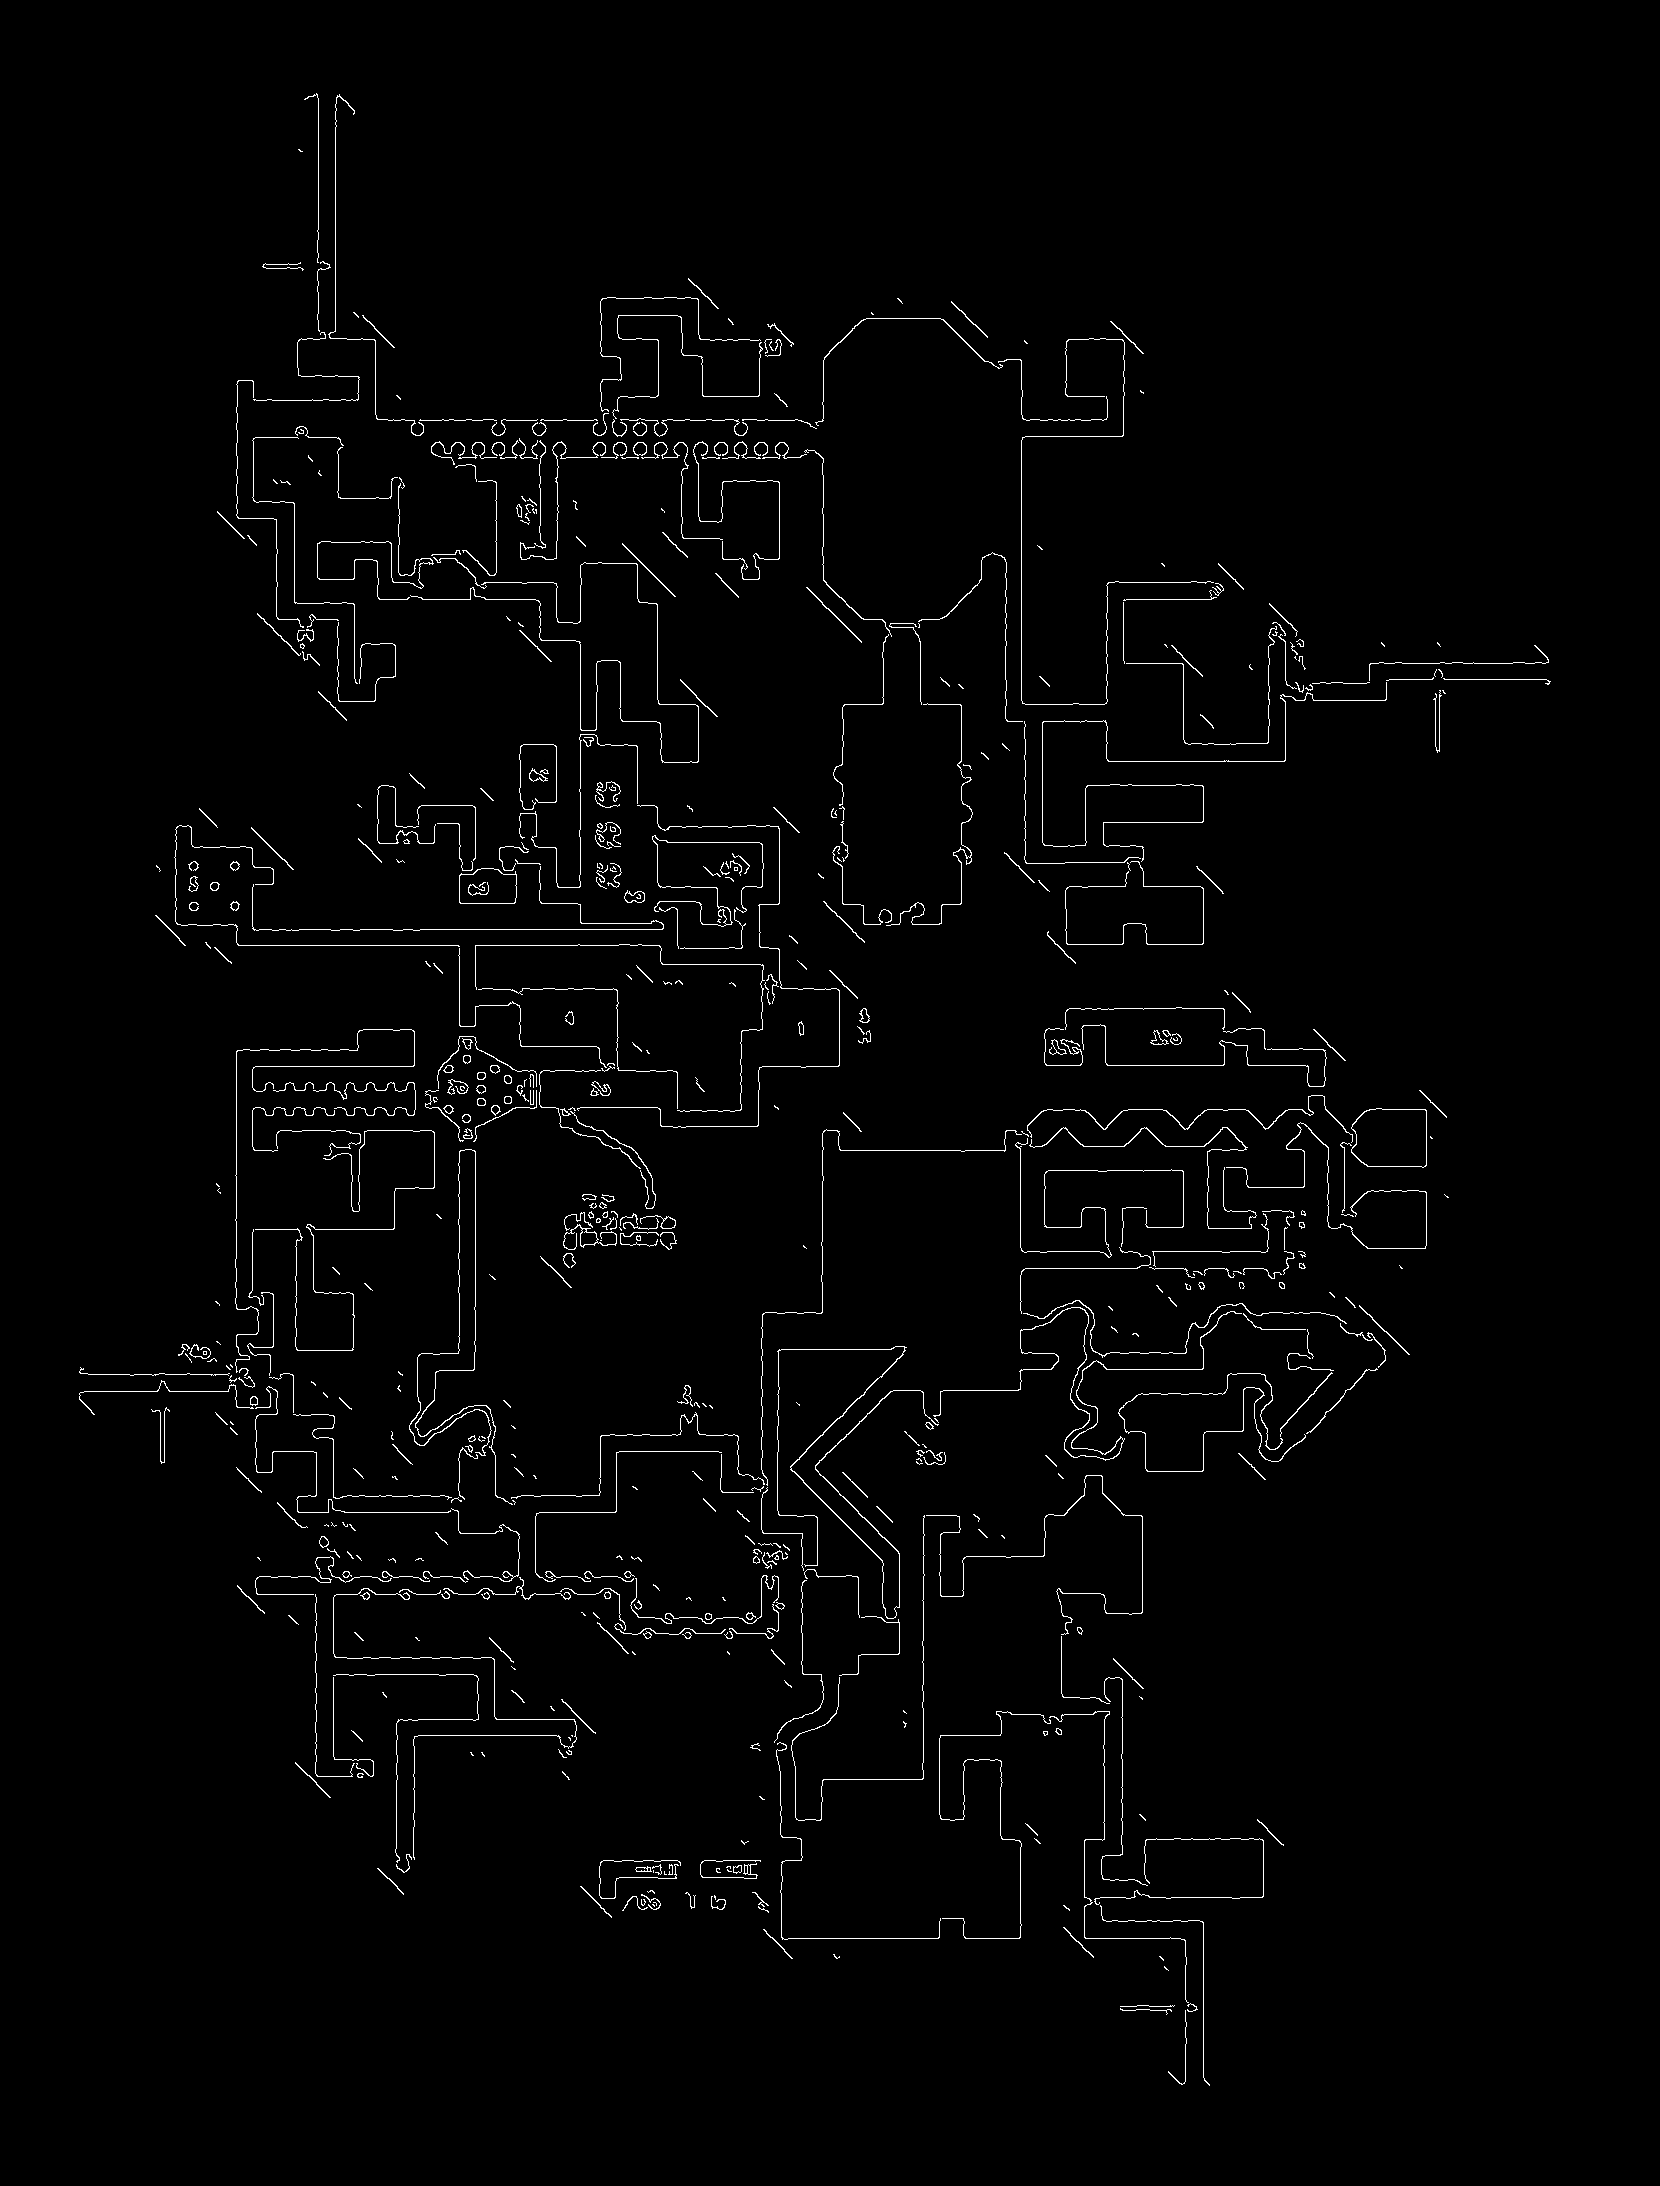
\includegraphics[width=0.35\linewidth]{images/darragh_result.png}
    \caption{Dungeon map border extraction example}
\end{figure}
\end{frame}


\section{Object detection with HAAR cascade classifiers}
\begin{frame}{Object detection with HAAR cascade classifiers}
\begin{block}{What is object detection ?}
	The ability to detect individual objects within an image.
	\begin{figure}
    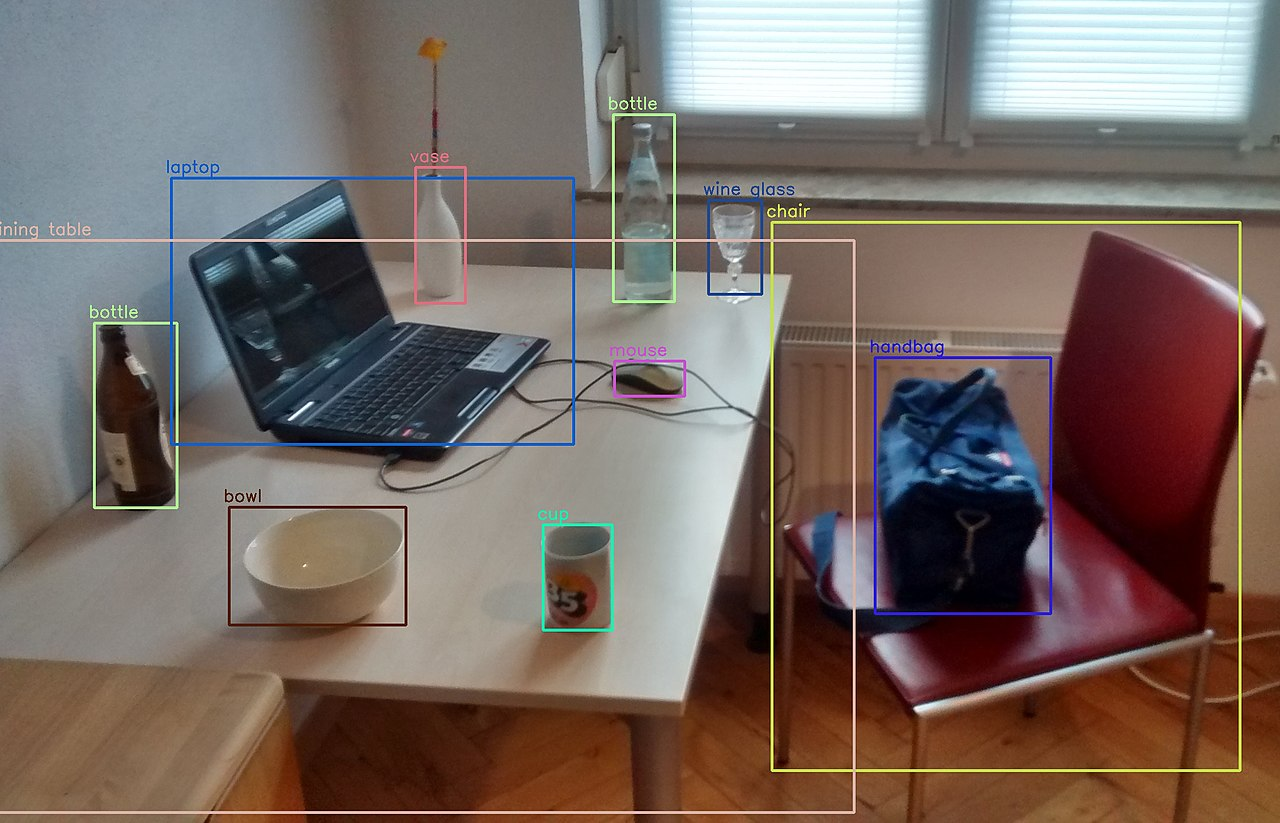
\includegraphics[width=0.35\linewidth]{images/obj_det_1.jpg}
\end{figure}
\end{block}
It is very hard because : 
\begin{itemize}
	\item Objects vary within a class (think of the different dog breeds)
	\item Different angles of view
	\item Ambiguity in identification (even for a human : sword, katana, knife, dagger, ...)
	\item Light/clarity of the scene
	\item ...
\end{itemize}
\end{frame}

\subsection{What is HAAR cascade classifiers ?}
\begin{frame}{What is HAAR cascade classifiers ?}
As we saw in traditional machine learning algorithms, \textbf{features can be extracted} from an image and \textbf{injected into classifiers} to identify objects.
\begin{block}{HAAR cascade classifiers}
\begin{itemize}
	\item Created by Paul Viola and Michael Jones in 2001 (also known as the Viola-Jones object detection framework)
	\item Cascade function is trained with positive/negative images
	\item Works only for a single class of object but can be used in parallel
	\item Is composed in 4 steps
\end{itemize}
\end{block}
\end{frame}
\begin{frame}{First step : HAAR feature selection}

\begin{itemize}
	\item Objects are classified using very simple feature
	\item Haar features are sequence of rescaled square shape functions proposed by Alfred Haar in 1909
	\item Each feature is defined by the difference of each pixel intensity within a defined pixel kernel.
\end{itemize}
\begin{figure}
    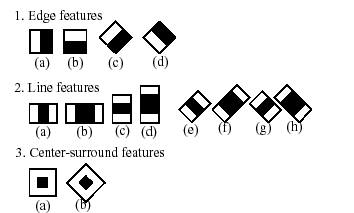
\includegraphics[width=0.5\linewidth]{images/haar_set.png}
\end{figure}
\end{frame}
\begin{frame}{First step : HAAR feature selection}

\begin{figure}[ht]
\begin{minipage}[b]{0.3\linewidth}
    \centering
    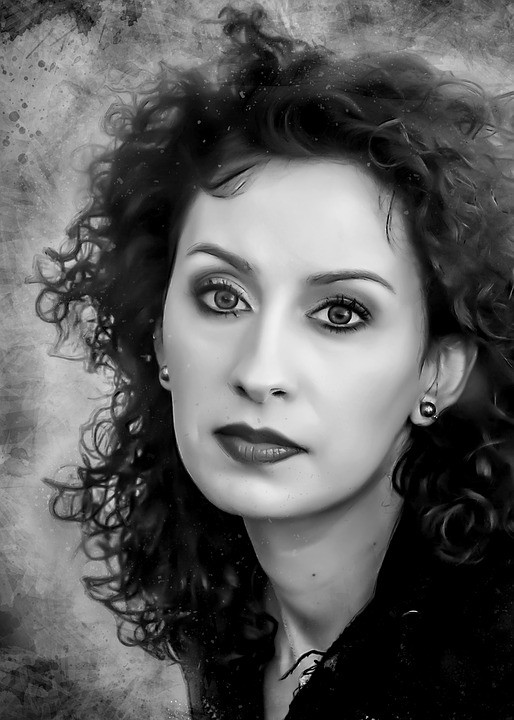
\includegraphics[width=\textwidth]{images/haar_feature_1.jpg}
    \caption{Original}
\end{minipage}
 \hspace{0.5cm}
\begin{minipage}[b]{0.3\linewidth}
    \centering
    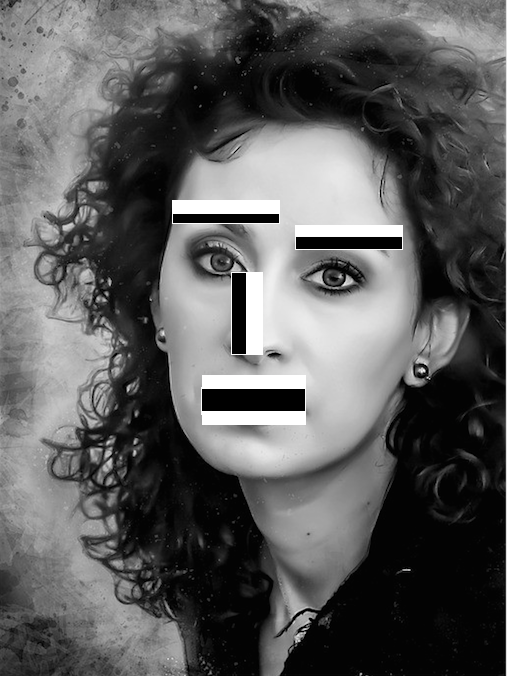
\includegraphics[width=\textwidth]{images/haar_feature_2.png}
    \caption{HAAR features on face}
\end{minipage}
\end{figure}

\end{frame}

\begin{frame}{Second step : Integral Image Representation}

\begin{itemize}
	\item The Value of any point is the sum of all the pixels above and left of that point.
	\item For 100X100 image, with a 9X9 window (slides 100 times) : 800 vs 356 operations
\end{itemize}
\begin{figure}[ht]
    \centering
    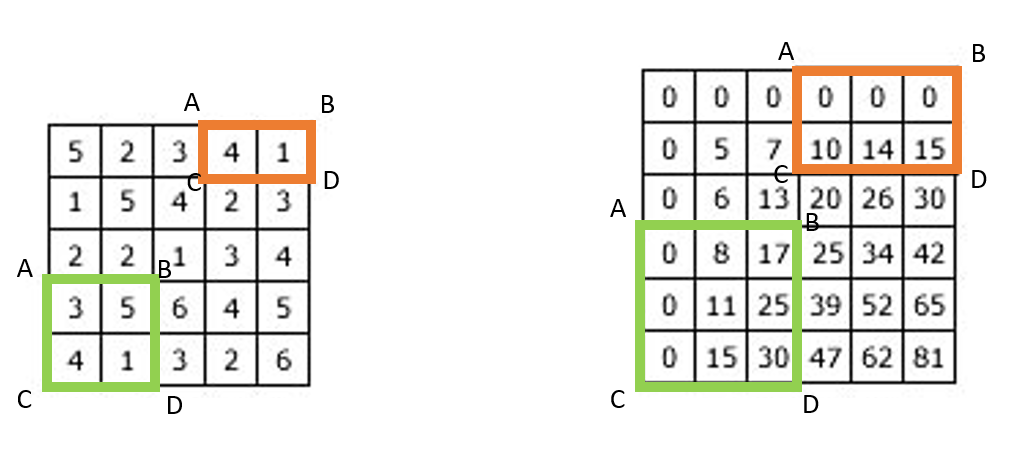
\includegraphics[width=0.5\textwidth]{images/integ_2.png}
    \caption{Original vs integral image representation}
\end{figure}
\begin{block}{The sum of each pixel in the window is simplified by}
\begin{equation}
\sum i(x,y) = I(D) + I(A) - I(B) -I(C)
\end{equation}
\end{block}
\end{frame}

\begin{frame}{Third step : Adaboost training}

\begin{itemize}
	\item All possible locations and size of each kernel is used to generate plenty features
	\item Using a 24X24 window size of the image will produce 160.000+ features
\end{itemize}
Wow that's a huge number, can we down size this ?
\begin{block}{Yes}
\begin{itemize}
  \item Most of the features are irrelevant
  \item Adaboost machine learning algorithm selects only the relevant ones : 160.000+ => 6000 features
\end{itemize}
\end{block}
\end{frame}

\begin{frame}{Fourth step : Cascade Classifier Architecture}
\begin{itemize}

\item Sliding a 24X24 window (generating 6000 features) over a 3.1 Megapixels image (120.000 times) would result into 72 million features.
\item Binary tree with successive classifier (strong -> weak) 
\item The quicker we can say "No" the better
\item On average only 3 evaluated features per window (72 M -> 360.000)
\item Generally we scale down the image with a 2/3 factor (360.000 -> 240.000)
\end{itemize}
\begin{figure}[ht]
    \centering
    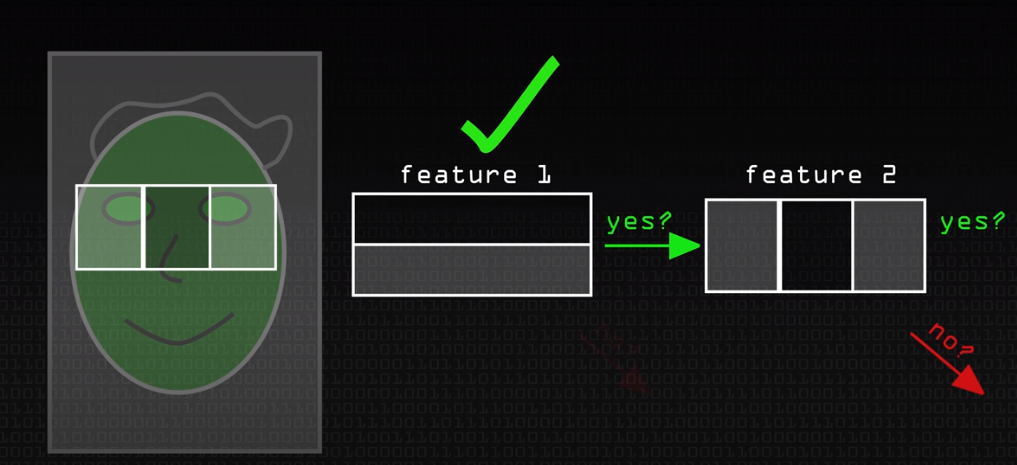
\includegraphics[width=0.6\textwidth]{images/haar_comp_1.png}
\end{figure}
\end{frame}


\subsection{Face and eye detection}
\begin{frame}{Face and eye detection}
Let's use two pre-trained face and eye HAAR cascade classifiers in parallel with OpenCV.
\end{frame}

\section{Object classification with Convolutional Neural Network}

\begin{frame}{Brief history of neural networks}
\begin{figure}[ht]
    \centering
    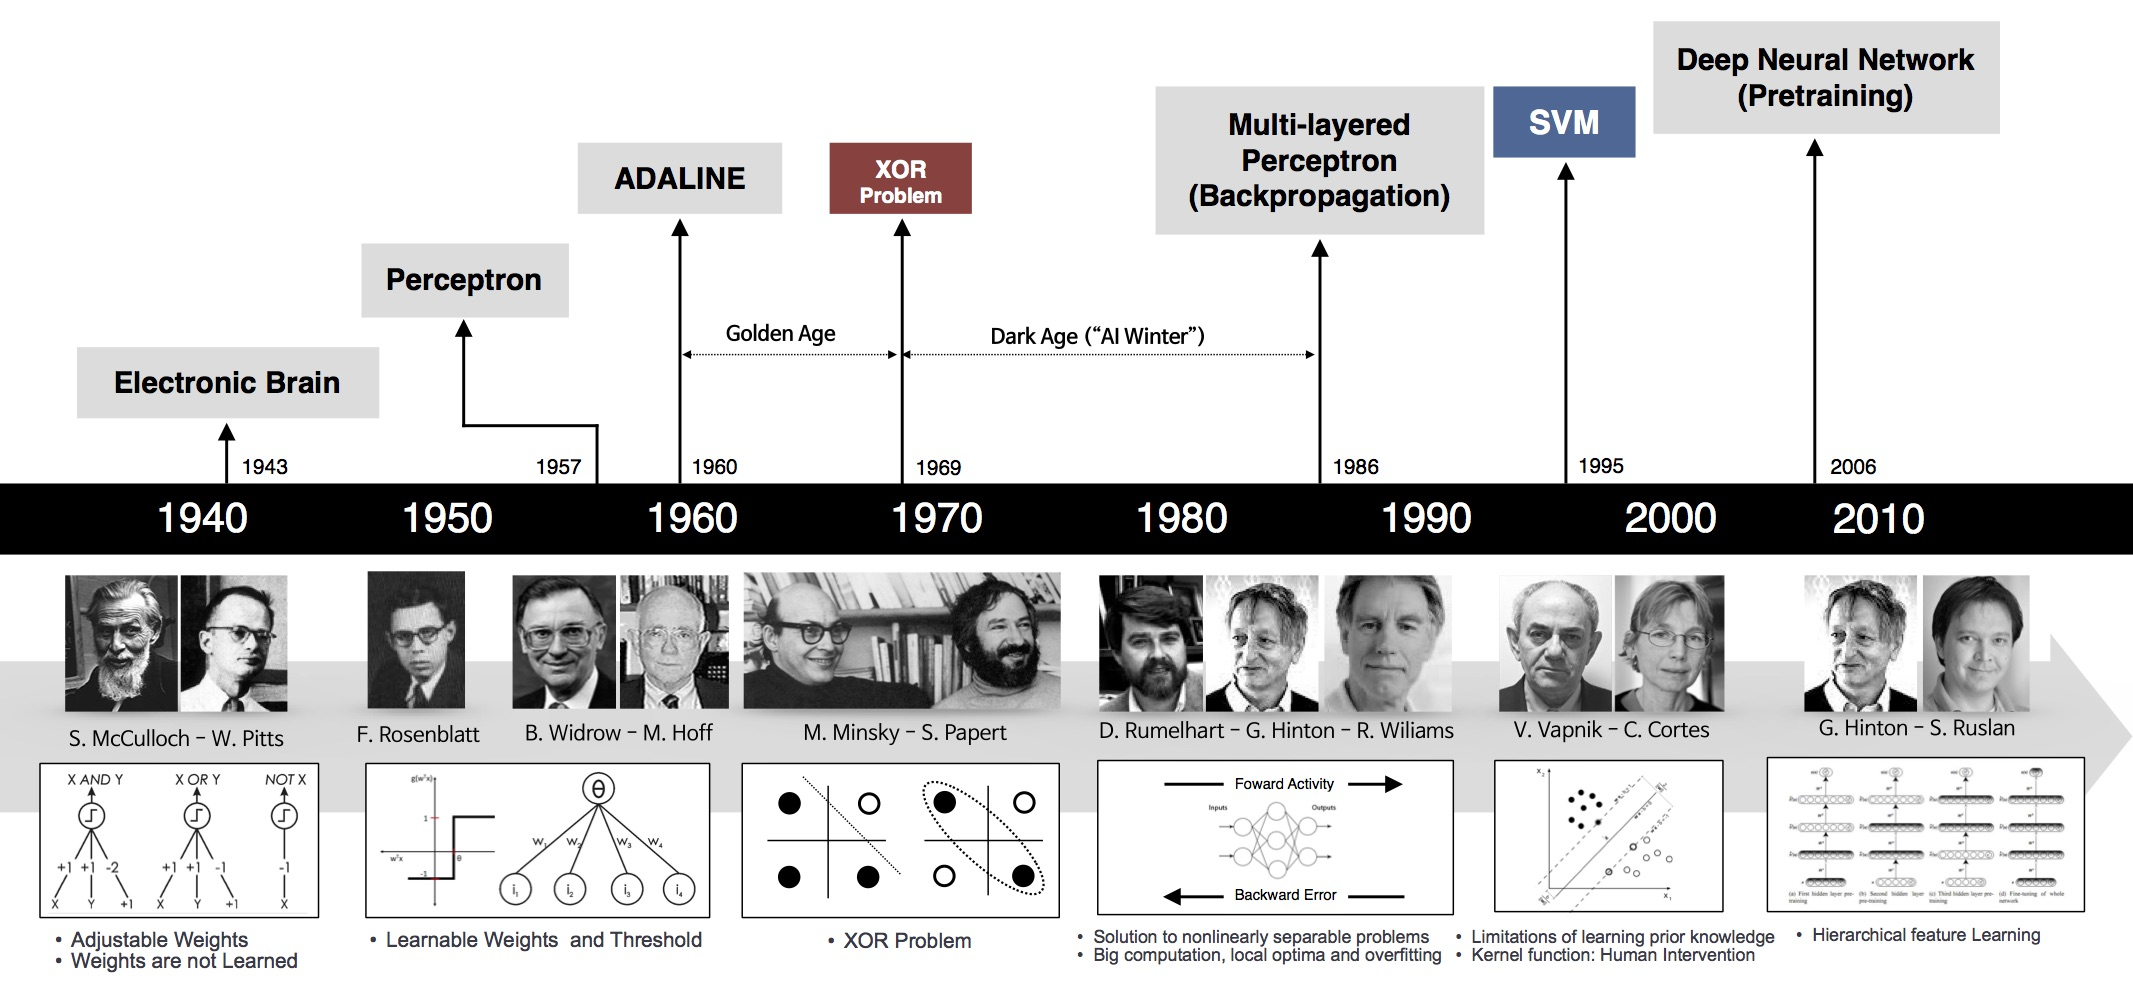
\includegraphics[width=0.9\textwidth]{images/deeplearning_2.png}
\end{figure}
Deeplearning was not possible in the 90's :
\begin{itemize}
\item Not enough labeled data or no solution to store them
\item Computers were too slow
\end{itemize}
\end{frame}

\begin{frame}{Neural network vs deeplearning}
\begin{figure}[ht]
    \centering
    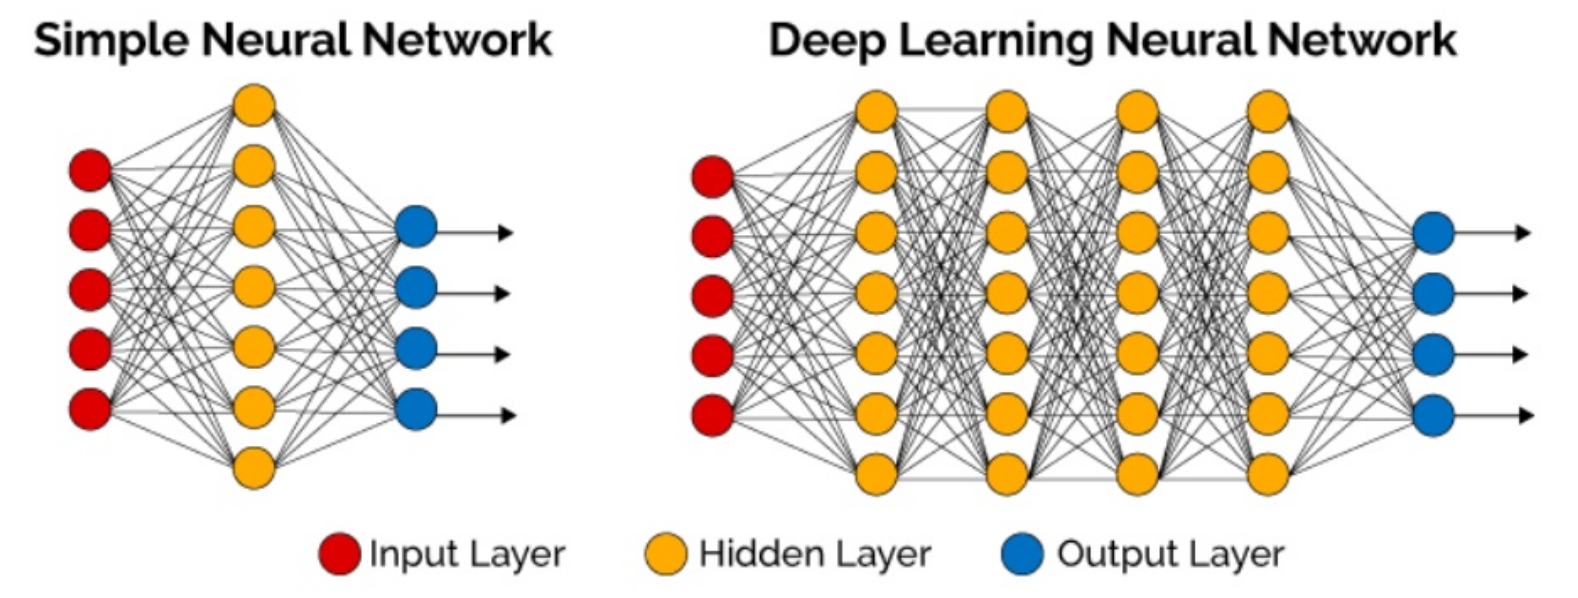
\includegraphics[width=\textwidth]{images/deeplearning_1.png}
\end{figure}
\end{frame}

\begin{frame}{What is a neuron ?}
\begin{figure}[ht]
    \centering
    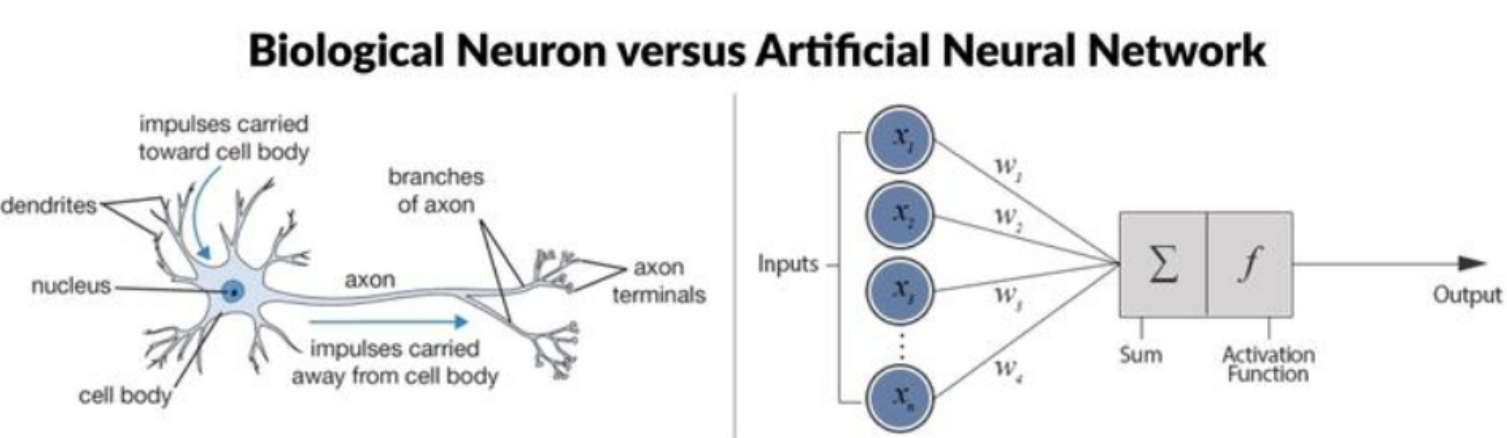
\includegraphics[width=\textwidth]{images/deeplearning_3.png}
\end{figure}
\end{frame}

\begin{frame}{The different activation functions}
\begin{figure}[ht]
    \centering
    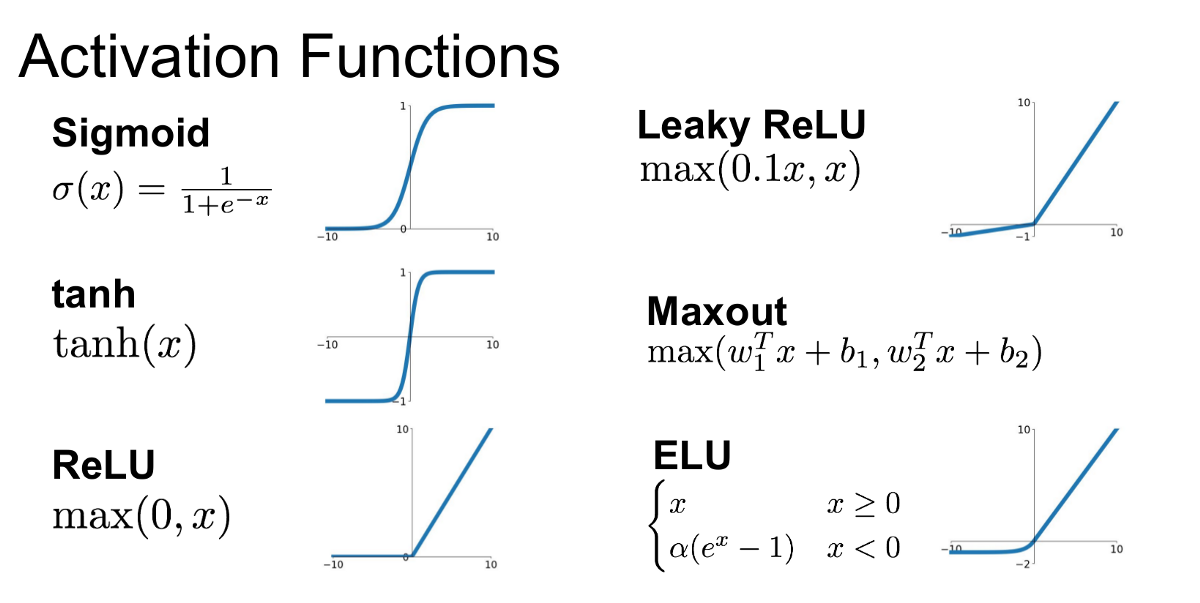
\includegraphics[width=\textwidth]{images/deeplearning_4.png}
\end{figure}
\end{frame}
\begin{frame}{Neural network training}
\begin{figure}[ht]
    \centering
    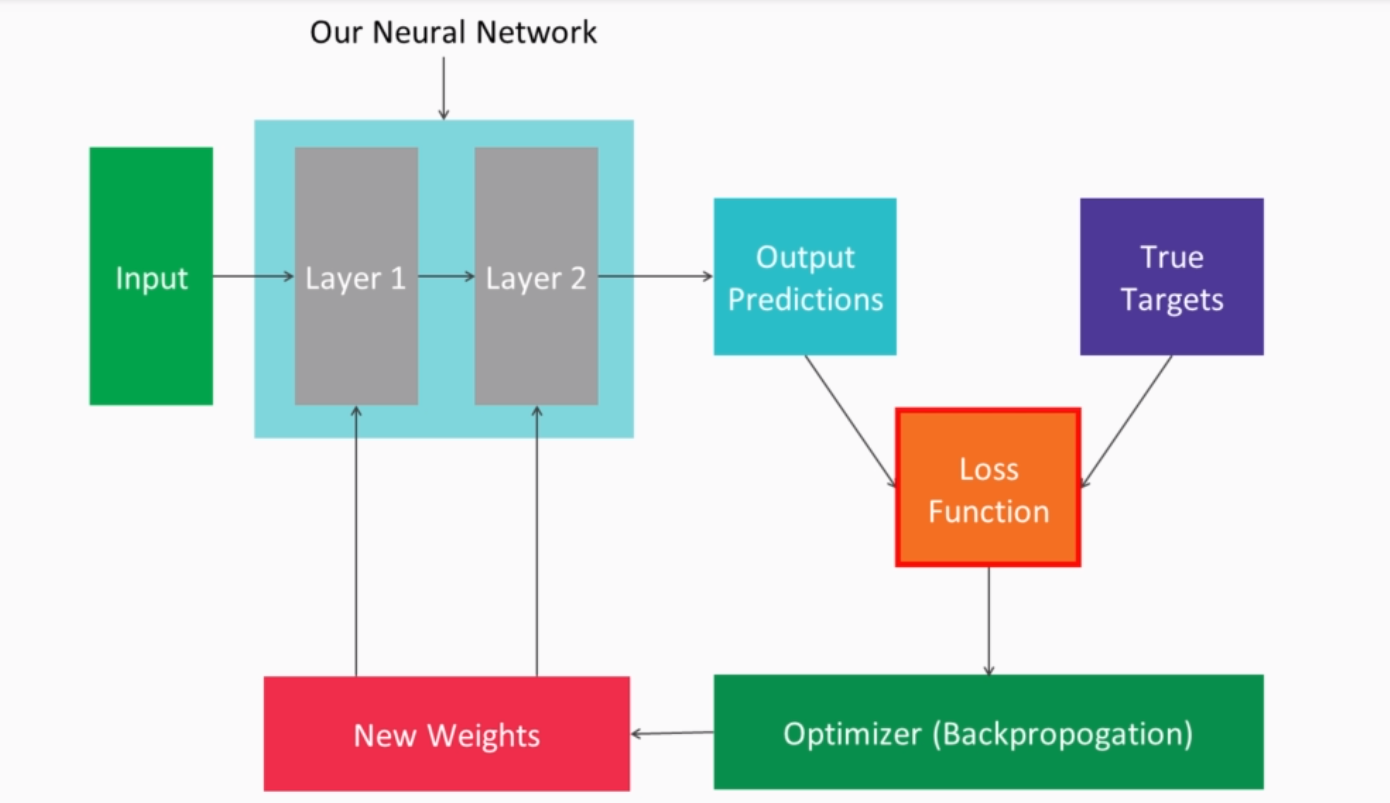
\includegraphics[width=\textwidth]{images/training_deeplearning.png}
\end{figure}
\end{frame}
\begin{frame}{Neural network training : Backpropagation}
    \animategraphics[loop,autoplay,width=\linewidth]{30}{images/animated_backpropagation/deeplearing-}{0}{99}
\end{frame}
\begin{frame}{Neural network training : Gradient descent}
    \animategraphics[loop,autoplay,width=\linewidth]{30}{images/animated_gradient_descent/gradient_descent-}{0}{96}
\end{frame}
\subsection{Convolutional Neural Network}

\begin{frame}{Convolutional Neural Network}
\begin{itemize}
  \item Take a colorized 680X480 image, the input of our NN is 680X480X3 = 979.200 weights !
\end{itemize}
\begin{block}{Are all the pixels value unrelated ?}
	No :
\begin{itemize}
  \item There are patterns through colors, edges, contours, ...
  \item All pixels are listed next to each other (spatially related)
\end{itemize}
\end{block}
\end{frame}
\begin{frame}{Convolutional Neural Network}
\begin{center}
    \animategraphics[loop,autoplay,width=0.75\linewidth]{2}{images/animated_kernel_1/kernel-}{0}{8}
    \animategraphics[loop,autoplay,width=0.5\linewidth]{5}{images/animated_kernel_2/kernel-}{0}{18}
\end{center}
\end{frame}
\begin{frame}{Convolutional Neural Network}
\begin{figure}[ht]
    \centering
    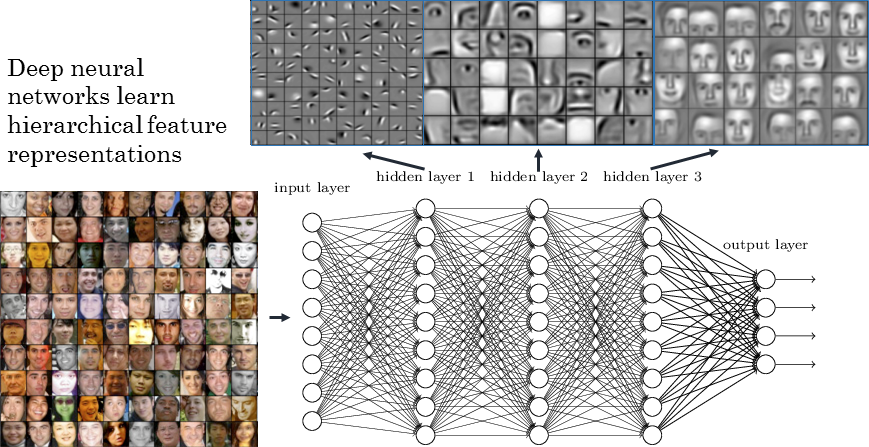
\includegraphics[width=0.75\textwidth]{images/hier_feature.png}
\end{figure}
\end{frame}

\begin{frame}{Convolutional Neural Network : Standard architecture}
\begin{figure}[ht]
    \centering
    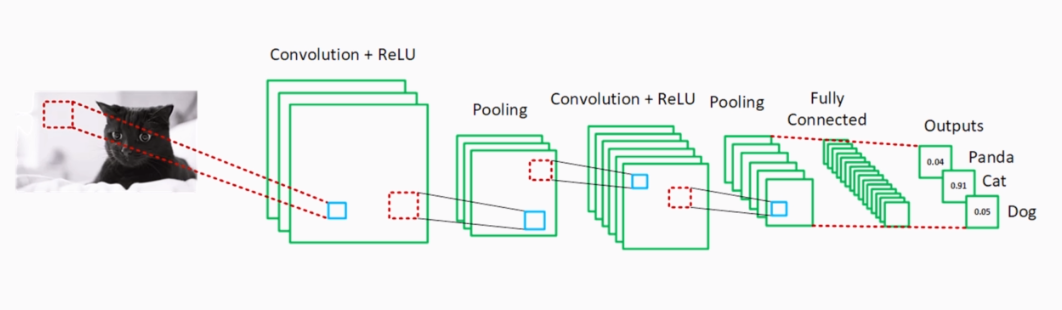
\includegraphics[width=0.75\textwidth]{images/architecture_1.png}
\end{figure}
\begin{itemize}
  \item Input
  \item Convolution + ReLU (Rectified Linear Unit) layer
  \item Pool layer (downsampling/subsampling layer)
  \item Fully connected layer (dense layer)
\end{itemize}
\end{frame}
\begin{frame}{Convolutional Neural Network : Standard architecture}
\begin{figure}[ht]
    \centering
    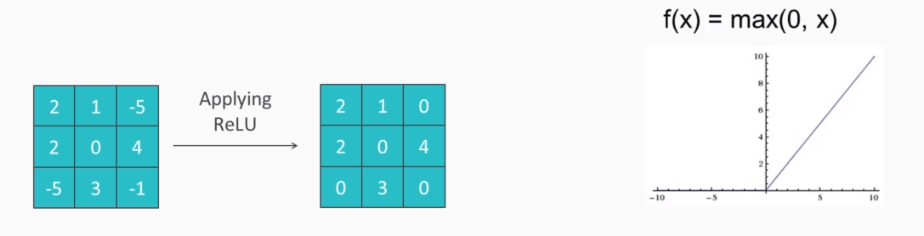
\includegraphics[width=0.75\textwidth]{images/relu.png}
\end{figure}
\begin{figure}[ht]
    \centering
    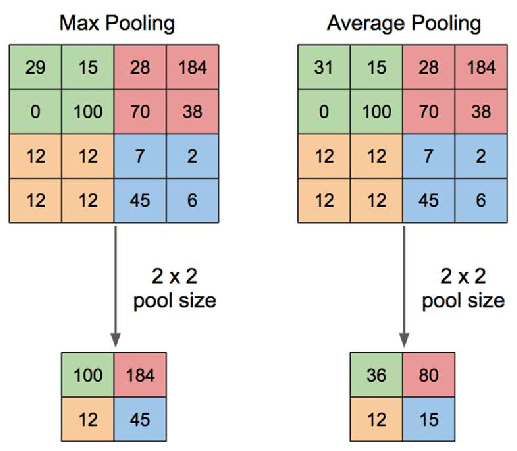
\includegraphics[width=0.4\textwidth]{images/pooling.png}
\end{figure}
\end{frame}

\begin{frame}{Convolutional Neural Network : Last problem, Overfitting}
\begin{figure}[ht]
    \centering
    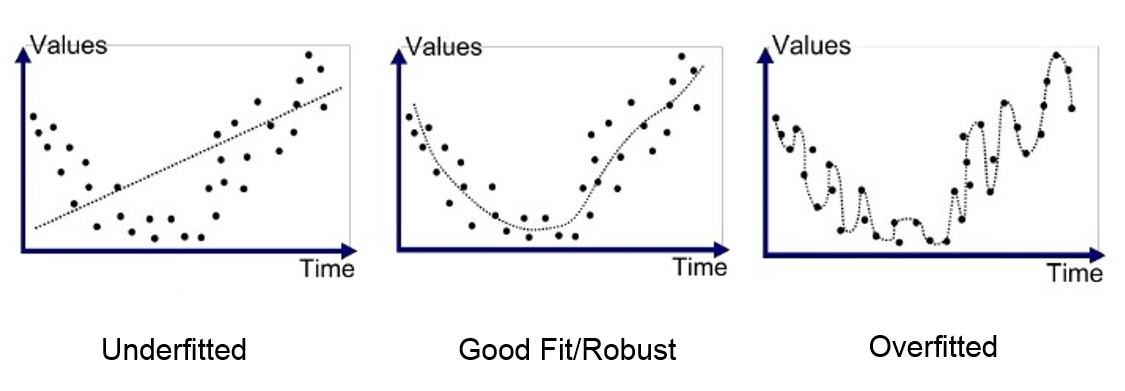
\includegraphics[width=0.75\textwidth]{images/overfitting_1.png}
\end{figure}
\begin{block}{Regularization methods}
\begin{itemize}
  \item Dropout (dropping nodes) => ignore some parts of the NN (during training)
  \item Penalize large weights (L1, L2 techniques)
  \item Cross validation (K-fold technique) - rotating test/train data
  \item Early stopping of the training
  \item Data augmentation (can be done artificially by flipping image e.g)
\end{itemize}
\end{block}
\end{frame}
\begin{frame}{Convolutional Neural Network : Designing tips}
\begin{itemize}
 \item Input layer: should be a square (no more than 64x64x3 => resize images)
 \item Input layer: should be divisible by 4 (for downsampling)
 \item Conv layer : stride (step for kernel movement) is 1 or 2, padding is 0 (so that output size = input size)
  \item Conv layer : minimum 2 layers
 \item Pool layer : generally 2x2 kernel
 \item Dense layer : activation function : 2 classes => sigmoid / 2+ classes => softmax
 \item Loss function :  2 classes => binary cross entropy / 2 + classes => Mean Squared Error (MSE)
 \item Gradient descent : use Stochastic Gradient Descent (SGD)
 \item Use dropout (very efficient against overfitting)
 \item Limit batch size if you run low on RAM
 \item Do 50+ epochs (iteration != epoch)
 \item Flow is : Input -> (Conv -> ReLU -> Pool) * X -> Dense -> Output
\end{itemize}
\end{frame}

\subsection{Building a face mask detector with custom CNN}
\begin{frame}{Building a face mask detector with custom CNN}
Let's create a CNN powered face mask detector (with Keras, high-level framework on top of TensorFlow)

\end{frame}

\section{Object detection with YOLO}
\begin{frame}{Object detection}
Object detection is the Graal of computer vision, it involves both object classification and localization.
\begin{figure}[ht]
    \centering
    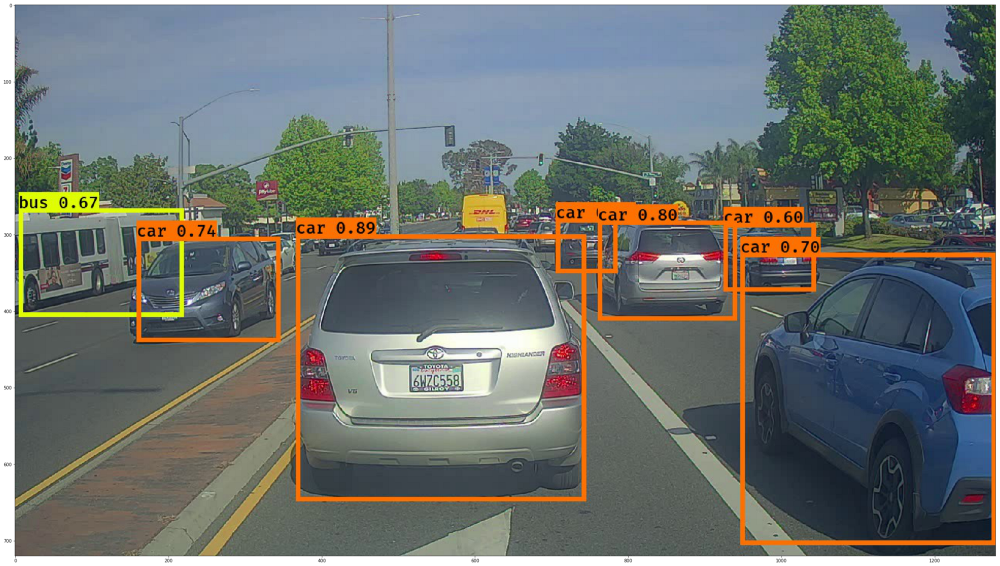
\includegraphics[width=0.9\textwidth]{images/obj_det_1.png}
\end{figure}
\end{frame}

\begin{frame}{Object detection with R-CNN}
A first attempt at doing object detection involving deep learning was the R-CNN (2014) algorithm (Regional Convolutional Neural Network).\newline


The algorithm is split in two parts :
\begin{itemize}
  \item Find the objects in the image via Selective Search Algorithm (determine contours in image)
  \item Inject the content of each box in a CNN to classify what's in the box
\end{itemize}
\begin{alertblock}{It was slow}
 A few slightly better attempts were made with same 2-steps concept
\begin{itemize}
\item Fast R-CNN  (2015)
\item Faster R-CNN (2016)
\end{itemize}
\end{alertblock}
\begin{figure}[ht]
    \centering
    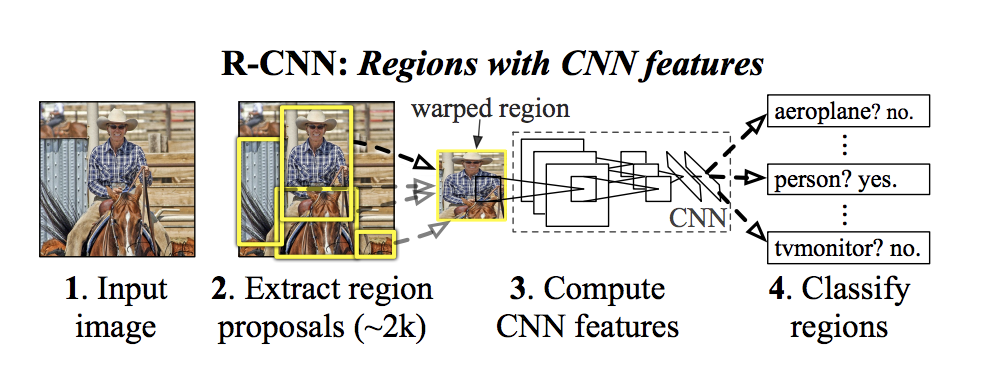
\includegraphics[width=0.5\textwidth]{images/r-cnn.png}
\end{figure}
\end{frame}

\begin{frame}{Object detection with YOLO}
Then YOLO cames in (2016) with the idea of doing both the box prediction + classification at once in the same neural network (You Only Look Once).
\begin{figure}[ht]
        \begin{minipage}[b]{0.35\linewidth}
            \centering
            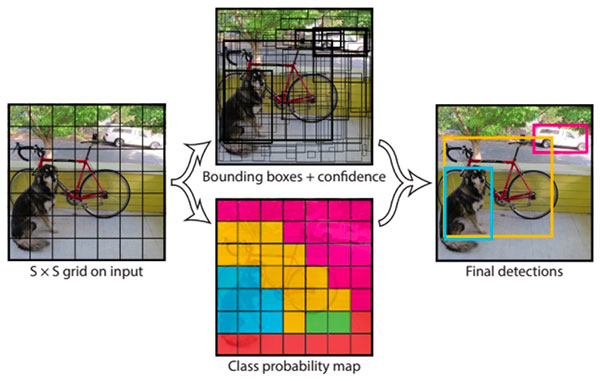
\includegraphics[width=\textwidth]{images/yolo_1.jpg}
            \label{fig:a}
        \end{minipage}
        \hspace{0.5cm}
        \begin{minipage}[b]{0.35\linewidth}
            \centering
            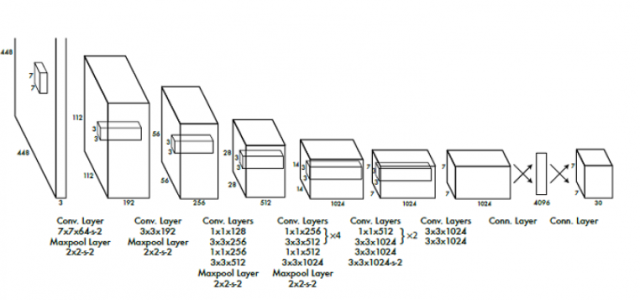
\includegraphics[width=\textwidth]{images/yolo_2.png}
            \label{fig:b}
        \end{minipage}
\end{figure}


It has since then been enhanced
\begin{itemize}
 \item YOLO 2 (2017) : high resolution support (448X448)
 \item YOLO 3 (2018) : multi-scale training for small objects detection
\end{itemize}
\end{frame}

\begin{frame}{Object detection with YOLO}
Let's use YOLO to do some object detection
\end{frame}

\begin{frame}{Thank you}
\begin{figure}[ht]
    \centering
    
\includegraphics[width=0.8\textwidth]{images/end.png}
\end{figure}
\end{frame}
%----------------------------------------------------------------------------------------

\end{document} 